\upshape
\index{Web Frontend}
\subsection{Introduction}
The Web Frontend provides access to experiment information and analysis tools in a read-only manner
and accessible by a web browser.

\subsection{System requirements}
\label{wfSR}
\index{System requirements, Web Frontend}
The web frontend is implemented as Python WSGI web application and makes use of several libraries.
Since it interfaces with R to draw plots it also depends on R and a Python interface to R, which unfortunately
only works properly on Linux right now.
WSGI applications can be deployed on a variety of web servers or even run standalone on a web server that comes with the
Python standard library.
The following list contains all dependencies and prerequisites of the Web Frontend (see \ref{wf:installation} for installation instructions).
\begin{itemize}
\item Python 2.6.5 or 2.7 http://www.python.org
\item R 2.11 (language for statistical computing and graphics)
\item R package 'np' (available via R's CRAN)
\item SQLAlchemy 0.6.5 (SQL Toolkit and Object Relational Mapper)
\item mysql-python 1.2.3c1 (Python MySQL adapter)
\item Flask 0.6 (Micro Webframework)
\item Flask-WTF 0.3.3 (Flask extension for WTForms)
\item Flask-Actions 0.5.2 (Flask extension)
\item Werkzeug 0.6.2 (Webframework, Flask dependency)
\item Jinja2 2.5 (Template Engine)
\item PyLZMA 0.4.2 (Python LZMA SDK bindings)
\item rpy2 2.1.4 (Python R interface)
\item PIL 1.1.7 (Python Imaging Library)
\item Numpy 1.5.1
\item pygame 1.9 (Graphics library)
\end{itemize}

\subsection{Installation}
\label{wf:installation}
\index{Installation, Web Frontend}
To get rpy2 working the GNU linker (ld) has to be able to find libR.so. Add the folder containing
libR.so (usually /usr/lib/R/lib) to the ld config: Create a file called R.conf containing the
path in the folder /etc/ld.so.conf.d/ and run ldconfig without parameters as root to update.
Additionally, you have to install the R package 'np' which provides non-parametric statistical
methods. This package can be installed by running ''install.packages('np')'' within the R interpreter (as root).

The following installation example outlines the step that have to be taken to install the web frontend on Ubuntu 10.04
running on the Apache 2.2.14 web server. For performance reasons (e.g. query latency) the web frontend should run on the
same machine that the EDACC database runs on.
\marginlabel{\Eexample}
\begin{enumerate}
\item Install Apache and the WSGI module: \begin{verbatim}apt-get install apache2 libapache2-mod-wsgi\end{verbatim}
\item{ Copy the web frontend files to /srv/edacc\_web/, create an empty error.log file and change their ownership to the Apache user: 
\begin{verbatim}
  touch /srv/edacc_web/error.log
  chown www-data:www-data -R /srv/edacc_web
\end{verbatim}
}
\item{ Create an Apache virtual host\\
(new file at /etc/apache2/sites-available/edacc\_web)
\begin{verbatim}
<VirtualHost *:80>
  ServerAdmin email@email.com
  ServerName foo.server.com

  LimitRequestLine 51200000

  WSGIDaemonProcess edacc processes=1 threads=15
  WSGIScriptAlias / /srv/edacc_web/edacc_web.wsgi

  Alias /static/ /srv/edacc_web/edacc/static/

  <Directory /srv/edacc_web>
    WSGIProcessGroup edacc
    WSGIApplicationGroup %{GLOBAL}
    Order deny,allow
    Allow from all
  </Directory>

  <Directory /srv/edacc_web/edacc/static>
    Order allow,deny
    Allow from all
  </Directory>
</VirtualHost>
\end{verbatim}
}
\item{Install dependencies and create a virtual environment for Python libraries:
\begin{verbatim}
apt-get install python-pip python-virtualenv python-scipy
apt-get install python-pygame python-imaging
virtualenv /srv/edacc_web/env
apt-get build-dep python-mysqldb
apt-get install r-base
echo "/usr/lib/R/lib" > /etc/ld.so.conf.d/R.config
ldconfig
source /srv/edacc_web/env/bin/activate
pip install mysql-python
pip install rpy2
pip install flask flask-wtf flask-actions
pip install sqlalchemy pylzma numpy
\end{verbatim}
}
\item{Install R libraries (''R'' launches the R interpreter):
\begin{verbatim}
R
install.packages('np')
\end{verbatim}
}
\item{Create a WSGI file at /srv/edacc\_web/edacc\_web.wsgi with the following contents:
\begin{verbatim}
import site, sys, os
site.addsitedir('/srv/edacc_web/env/lib/python2.6/site-packages')
sys.path.append('/srv/edacc_web')
sys.path.append('/srv/edacc_web/edacc')
os.environ['PYTHON_EGG_CACHE'] = '/tmp'
sys.stdout = sys.stderr
from edacc.web import app as application
\end{verbatim}
}
\item Configure the web frontend by editing /srv/edacc\_web/edacc/config.py, see~\ref{wf:configuration} for details.
\item{Enable the Apache virtual host created earlier:
\begin{verbatim}
a2ensite edacc_web
service apache2 restart
\end{verbatim}
}
\item The web frontend should now be running under http://foo.server.com/
\end{enumerate}

\subsection{Configuration}
\label{wf:configuration}
\index{Configuration, Web Frontend}
All configuration is done in a Python file located at ''edacc/config.py''. The options are documented in the sample configuration
file which is included in the distribution package. Please read through the configuration options and modify those marked as important. \attention
Most importantly, you should disable debugging mode and change the secret key when making the Web Frontend
accessible from the network to avoid security problems. Logging is also quite useful to make it easier to find the cause of bugs in the application.
\marginlabel{Database configuration}At the end of the file you can configure the database connection and the list of EDACC databases that should be
made available by the Web Frontend.

\subsection{Troubleshooting}
\label{wf:troubleshooting}
\index{Troubleshooting, Web Frontend}
When there are errors or bugs and you have set up the Web Frontend under Apache as described in the installation section, Apache will display an ''Internal Server Error'' page.
If you have configured logging, the application will write tracebacks to the logging file. If you haven't set up logging, these tracebacks will end up
in Apache's error.log file.

\subsection{Features}
This section gives a short overview of the features of the Web Frontend. Most features should be self-explanatory or have some additional documentation
on the pages themself.

The Web Frontend was designed as monitoring and analysis tools of experiments that are created with the GUI application. Once you have set up some databases and added
them to the configuration file of the Web Frontend, the top level page will allow the user to select one of the databases. This leads to a page that displays
all experiments of the chosen database and some basic information about their creation date, number of solvers, instances and jobs.

\marginlabel{Experiments}
An experiment page displays further information about the experiment, such as the number of total, running and crashed jobs. If the experiment is currently
being computed, an estimation of the time of completion is displayed next to ''ETA''.

\marginlabel{Monitor progress}
Under ''Progress'' a colored bar visualizes the computation progress.
Green color corresponds to finished jobs, red to crashed jobs and orange to jobs that are currently being computed. The links following the progress bar
lead to information and analysis pages.

\index{Computation progress, Web Frontend}
\marginlabel{Job browser}
The progress page provides a job browser similar to the GUI application. It allows to sort, filter for certain words, show and hide specific columns and download
currently displayed data in CSV (comma-separated values) format\marginlabel{Export data}. Displaying more than 1000 results at once can become rather slow, since the browser's Javascript
engine has to do a lot of processing to color and format the table.

The solver configurations and instances pages show the solver configurations and instances that are part of the experiment. The instances page provides a download link
for all instance files in a tarball\marginlabel{Download instances}.
Instances are shown in a table by name, MD5 checksum and their properties (TODO reference), if there are any. The instance name links to a page that displays the 
first and last few characters of the instance file and provides a download link.

\marginlabel{View results}
\index{Results}
\index{Export results}
The result pages display the results of the jobs in various formats. ''Unsolved instances'' and ''Solved instances'' list the instances that
were not solved by any solver or solved by at least one solver respectively. ''By solver configuration'' leads to a page, where after selecting a solver configuration
that is part of the experiment a table is displayed containing all the results of the jobs of the solver configuration by instance and run number.
''By instance'' leads to a page, where after selecting an instance all results obtained on this instance are displayed by solver configuration and run number.
\marginlabel{Export results}All tables can be exported (i.e. downloaded) in CSV format.

\marginlabel{Analyse results}
\index{Analysis}
\index{Statistical tools}
\index{Visualization}
\index{Plots}
Analysis pages provide various plots of results and statistical tools such as correlation and probabilistic domination calculations. All plots can be directly saved
in PNG format as they are displayed in the browser or downloaded in PDF or EPS format\marginlabel{Export plots}\index{Export plots}. For some plots the application generates an R script which can be adjusted as
neccessary.
Most plots allow to download the underlying data in CSV format.

Some plots allow the selection of multiple instances. In this case, you can use a filter to narrow the selection of the instances listed. Please refer to the example
which is displayed next to the filter text field.

\marginlabel{Ranking of solver configurations}
\index{Ranking}
The ranking is determined by the number of successful runs but the ranking table can be sorted by any of the displayed measures.


\subsection{Result pages}
\begin{figure}
\centering
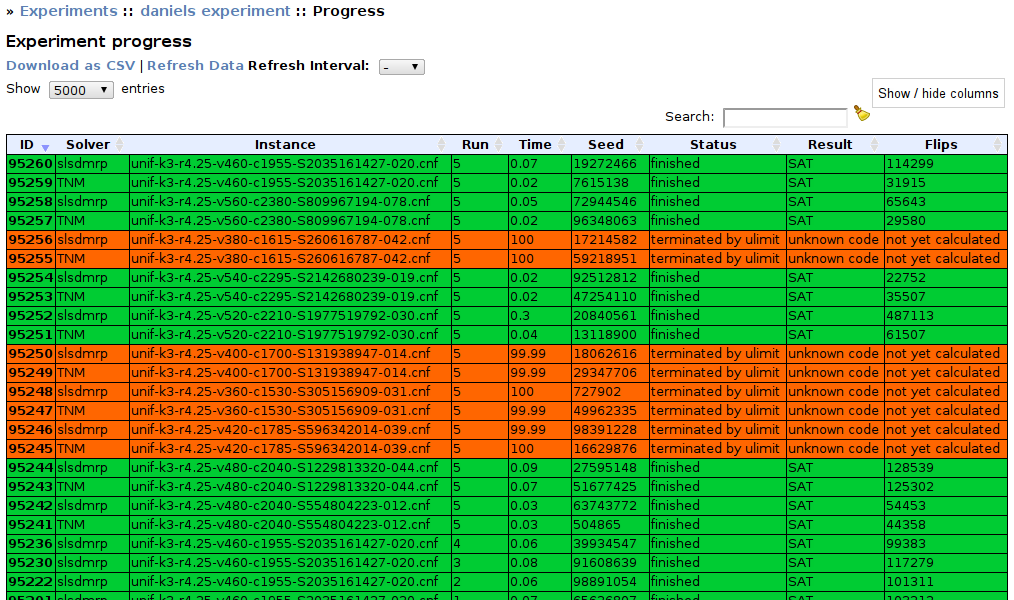
\includegraphics[width=8cm]{progress_table.png}
\caption{Live result browser showing the jobs of an experiment on SAT solvers. The ''Flips'' result property column contains the values of the number of local search steps performed by the solver.}
\label{fig:progress_table}
\end{figure}
The main web page gives a list of experiments that are in the database along with information about the experiment's date, number of solver configurations, instances and attempts.
Each experiment in the list links to a web page that provides links to various web pages with further information, results and analysis tools.

The \emph{Live information about experiment progress} page displays a table of the experiment's jobs in rows with several columns for the attributes of a job.
By default, the unique ID of a job, its solver configuration, instance and run number, run time, seed, status and result code in textual form, are displayed.
Additionally, for each result property in the database there's a column with the property value of the job, if it was already calculated and is present in the database.
The job data is retrieved from the database on each page refresh and directly reflects the computation progress of an experiment.
Aside from browsing the table, which includes sorting and filtering for some of the columns, the table data can also be downloaded in CSV format\footnote{comma-separated values} for
processing with other tools.
The ID is also a link that leads to a \emph{detailed result} page for the job. This page displays links to the solver configuration and instance of the job and the values of all result properties, if they are calculated. The solver, launcher, watcher and verifier output is displayed as well but each truncated to a reasonable size, only showing the first and last few hundred
characters. Links allow the user to download the entire files.

The ''list of solver configurations used'' page displays the list of solver configurations that are part of the experiment. For each solver configuration
a page with details about the solver and the arguments can be accessed.
The ''list of instances used'' page displays the list of instances used in the experiment in a table. There are columns for the name, md5 checksum and additional columns for each
instance property defined in the database. Each instance has a link to a page that displays the first and last few hundred characters of the instance file and allows to download
the entire file.

There are three pages that display the results of an experiment in different formats:
\begin{enumerate}
\item By solver configuration: Allows the user to select a solver configuration and then displays a table with the solver configuration's run time results of all attempts on the instances
of the experiment. The results are links to the detailed result pages of the corresponding jobs.
\item By instance: Allows the user to select an instance and then displays a table with the run time results of all attempts of the solver configurations of the experiment.
\item By solver configuration and instance: Displays a table with the instances of the experiment as rows and the solver configurations as columns.
If there's only one attempt for each solver on an instance, the cell corresponding to a particular solver configuration and instance displays the
run time of the single attempt and it's result code in textual form. If there are multiple attempts, each cell contains descriptive statistics such as the
median, minimum, maximum and average run time, as well as its standard deviation, over all attempts. A link in each cell leads to a table with the results of all attempts.
\end{enumerate}
The data of the tables displayed in the two result pages mentioned first can be downloaded in CSV format.

\subsection{Analysis pages}
The statistical methods implemented were described in chapter \ref{chap:analysis} in detail. In the web frontend they are made available on pages that are accessible from an experiment's main page. Each has a form that allows the user to set the parameters of the plots and tests, for example which solver configurations and instances to include. After submitting the form the pages display the results of the tests or the plots.
\begin{figure}
\centering
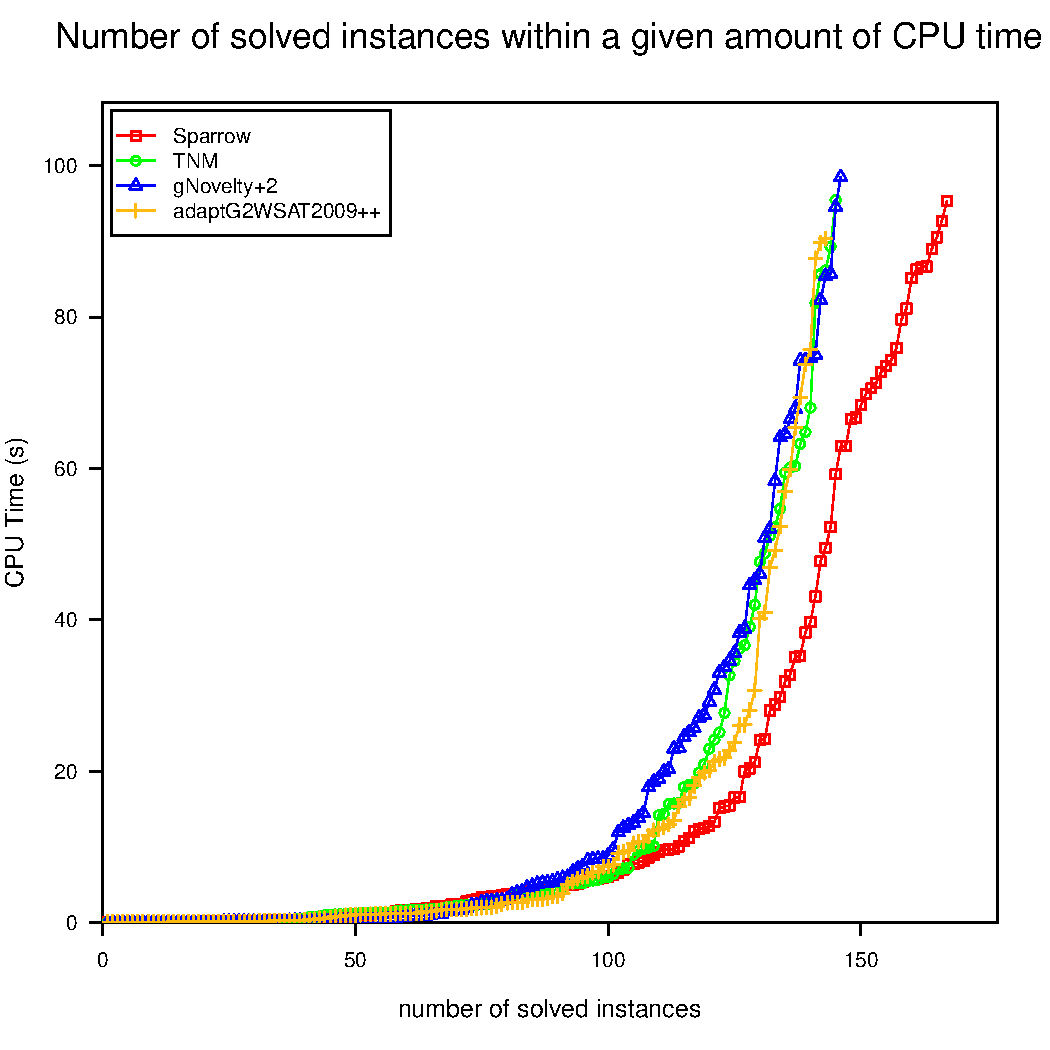
\includegraphics[width=9cm]{SAT_Competition_scenario_cactus}
\caption{Cactus plot}
\label{fig:cactus}
\end{figure}
The following tests and plots are implemented in the web frontend:
\begin{itemize}
\item Box plots: The form allows the selection of the result property and the solver configurations and instances of which the results should be plotted. After submitting the form the box plot is displayed.
\item Scatter plot - One result property of two solvers: The form allows the selection of the two solver configurations, the instances and whether to plot single runs, all runs or average or median values.
\item Scatter plot - Two result properties of a solver: The form allows the user to select the solver configuration, the instances and whether to plot single runs, all runs or average or median values.
\item Scatter plot - Result property against instance property: A form allows to select the solver configuration, result property, instance property and whether to plot single runs, all runs or average or median values.
\item Distribution and Kernel Density Estimation: After selecting the solver configuration, instance and result property the plots of the empirical distribution function and the kernel density estimation are displayed.
\item Property distribution comparison of two solvers on an instance: A form allows to select two solver configurations, the instance and the result property. After submitting the form data, a plot of both property distributions and the results of the two hypothesis tests described in the last chapter are displayed. For both tests, the null hypothesis, the alternative hypothesis, the test statistic, the p-value and the conclusion about whether to accept or reject the null hypothesis at significance level $0.05$ are calculated and displayed.
\item Property distributions of solvers on an instance: After selecting several solver configurations, an instance and a result property, the result property distributions are displayed in a single plot.
\item Cactus plot: Cactus plots show the number of attempts a solver configuration would be able to finish successfully if it is restricted to a certain amount of a result property on every attempt. For example, the number of successful runs if given a certain amount of time (see Figure~\ref{fig:cactus}).
\item Probabilistic domination: After selecting two solver configurations and a result property the instances are split into the three categories of probabilistic domination as described in chapter~\ref{chap:analysis}.
\end{itemize}
The \emph{Pearson product-moment correlation coefficient} and \emph{Spearman's rank correlation coefficient} are calculated for the data of the scatter plots and displayed next to them.
All plots are rendered in PNG\footnote{Portable Network Graphics} format for presentation on the web pages and can be downloaded by the user as PDF and EPS\footnote{Encapsulated Postscript} images
for further use. Additionally, the numeric data that is used to generate the plots can be downloaded in CSV format.
